\documentclass{article} % For LaTeX2e
\usepackage{iclr2022_conference,times}
% Optional math commands from https://github.com/goodfeli/dlbook_notation.
\input{math_commands.tex}

%######## APS360: Uncomment your submission name
\newcommand{\apsname}{Project Proposal}
%\newcommand{\apsname}{Progress Report}
%\newcommand{\apsname}{Final Report}

%######## APS360: Put your Group Number here
\newcommand{\gpnumber}{1}

\usepackage{hyperref}
\usepackage{url}
\usepackage{graphicx}

%######## APS360: Put your project Title here
\title{Pedestrian Trajectory Tracking  \\ 
Project Proposal}


%######## APS360: Put your names, student IDs and Emails here
\author{Tony Wang  \\
Student\# 1009027447\\
\texttt{tonyivt.wang@mail.utoronto.ca} \\
\And
Benjamin Low  \\
Student\# 1009022273 \\
\texttt{benjamin.low@mail.utoronto.ca} \\
\And
Joey Zou  \\
Student\# 1009080110 \\
\texttt{joe.zou@mail.utoronto.ca\hspace{45pt}} \\
\And
Jonathan Choi \\
Student\# 1009035599 \\
\texttt{jonny.choi@mail.utoronto.ca} \\
}

% The \author macro works with any number of authors. There are two commands
% used to separate the names and addresses of multiple authors: \And and \AND.
%
% Using \And between authors leaves it to \LaTeX{} to determine where to break
% the lines. Using \AND forces a linebreak at that point. So, if \LaTeX{}
% puts 3 of 4 authors names on the first line, and the last on the second
% line, try using \AND instead of \And before the third author name.

\newcommand{\fix}{\marginpar{FIX}}
\newcommand{\new}{\marginpar{NEW}}

\iclrfinalcopy 
%######## APS360: Document starts here
\begin{document}


\maketitle

----Total Pages: \pageref{last_page}

\section{Introduction}

Pedestrian trajectory tracking is a complex task that involves recognizing and following individuals from video footage. This problem is interesting as it requires solving several challenges: distinguishing people from the background, differentiating them from non-human objects, individually identifying each person, and consistently tracking individuals as they move.

The importance of accurate pedestrian tracking extends across several domains. For self-driving cars, the ability to detect and track pedestrians is fundamental for ensuring safe navigation, especially at intersections and on shared roads. Past trajectory is essential in developing models that predict pedestrian intent and their future actions: whether they will turn, cross, stop, etc. \citep{6632960}. In the development of smart cities, effective pedestrian tracking can enable advanced functionalities, from automatic traffic light control to detailed urban planning analytics. Furthermore, while pedestrian tracking has the potential for positive advancements, it also raises ethical concerns regarding mass surveillance. This topic will be explored in the ethics section of this proposal.

Traditional approaches to object tracking, such as background subtraction, temporal differencing, and optical flow, face significant challenges in complex environments. These methods struggle with variations in illumination, dynamic backgrounds, object occlusion, clutter, and video noise \citep{shaikh2014}. Deep learning is novel in its capability to identify high-level features and recognize complex patterns. Furthermore, multi-layered systems can learn the intrinsic characteristics of objects, allowing models to better track objects even in complex video \citep{jin2024}.

This project aims to use deep learning methods to overcome the traditional challenges and improve the accuracy and reliability of pedestrian trajectory tracking. Specifically, the goal is to produce a robust system capable of outputting the time-dependent trajectory of every human in-frame of every given stereo footage.

\section{Background and Related Work} \label{background}
\subsection{DeepSORT}
The paper ``Simple Online and Realtime Tracking with a Deep Association Metric'' \citep{wojke2017simple} integrates the appearance information using a convolutional neural network (CNN) trained on a large-scale person re-identification dataset. This method reduces identity switches by 45\%, enhancing tracking through occlusions by combining both motion and appearance data. The online tracking remains efficient and capable of real-time performance at the cost of increased pre-training complexity. Experimental results on the MOT16 benchmark demonstrate that DeepSORT achieves higher accuracy and robustness at high frame rates. 

\subsection{CityFlow}
The paper ``CityFlow: A City-Scale Benchmark for Multi-Target Multi-Camera Vehicle Tracking and Re-Identification'' \citep{tang2019cityflow} presents CityFlow, a dataset for urban traffic optimization. It includes over 3 hours of synchronized HD video from 40 cameras across 10 intersections, with more than 200,000 annotated bounding boxes. CityFlow features extensive spatial coverage, camera calibration information, and a subset for image-based vehicle re-identification (ReID). The dataset supports evaluations of MTMC tracking, single-camera tracking, object detection, and ReID, and aims to advance research in these areas. An evaluation server is available through the 2019 AI City Challenge. 
\subsection{Online Multi-Target Tracking Using Recurrent Neural Networks}
``Online Multi-Target Tracking Using Recurrent Neural Networks'' \citep{milan2016online} presents a pioneering method for online multi-target tracking utilizing recurrent neural networks (RNNs). Traditional multi-target tracking faces challenges such as varying target numbers and data association complexity. Unlike prior methods requiring complex models and parameter tuning, this approach offers end-to-end learning for multi-target tracking. Employing RNNs, it addresses challenges like continuous state estimation and discrete data association. Experiments on synthetic and real data demonstrate promising results, achieving approximately 300 Hz processing speed on standard CPUs. This work opens avenues for future research in online multi-target tracking, offering a principled solution to address real-world tracking challenges. 
\subsection{YOLO (You Only Look Once)}
YOLO (You Only Look Once) is a novel approach to object detection that treats the task as a regression problem. Unlike traditional methods that rely on classifiers, YOLO utilizes a single convolutional neural network to predict bounding boxes and class probabilities directly from full images in one pass. This unified architecture offers advantages such as real-time processing speeds, global reasoning about images, and generalizable representations of objects. While YOLO may exhibit more localization errors compared to some state-of-the-art systems, its simplicity and efficiency make it appealing for various applications, including autonomous driving and assistive devices. In contrast to traditional methods like DPM and R-CNN, YOLO's end-to-end approach and speed optimizations mark a significant advancement in object detection technology \citep{redmon2016look}.
\subsection{Learning Human Identity From Motion Patterns}
The paper ``Learning Human Identity from Motion Patterns'' by \citet{neverova2016} presents a method for biometric authentication using motion patterns captured by mobile sensors. They collected data from 1,500 volunteers and developed a model that extracts features using deep neural networks. Authentication is performed on-device for privacy reasons. They compare different neural network architectures and propose a dense convolutional clockwork recurrent neural network (DCWRNN) to address the limitations of existing models. 
\section{Data Processing}
\subsection{UCY Dataset}
We will use the UCY dataset, a video-based dataset in which pedestrians are tracked as they walk across a fixed camera. The video is taken at 2.5 Frames Per Second; frames contain labelled information on each pedestrian's $x$ and $y$ coordinates, as well as their gaze direction. The UCY dataset was first introduced by \citet{lerner2007ucy} to perform analysis on crowds; we, however, will use this dataset to train a neural network to predict the trajectories of pedestrians. This dataset was chosen over others as it only contains pedestrians, making identification easier. 

\subsection{Preprocessing}
Along with video files, the labels for each video can be found in a plaintext file, which follows the format included in Figure \ref{fig:enter-label}. The information on a specific pedestrian (each set of $N$ or $K$ control points) must be sorted and separated into individual arrays.
\begin{figure}[!h]
    \centering
    \includegraphics[width=0.5\linewidth]{Figs/read_me_ucy.png}
    \caption{The readme file in the UCY dataset shows how the pedestrian labels are formatted.}
    \label{fig:enter-label}
\end{figure}

The video files must also be preprocessed to be fed into the model. The model will have a set input layer size so the videos must be cropped and/or resized accordingly. This can be done with the tool \textit{FFmpeg} an open-source tool for processing video files.

\subsection{Dataset Link}

\url{https://github.com/Habiba-Amroune/ETH-UCY-Preprocessing}

\subsection{Further Data Collection}
Given the ease with which pedestrian trajectory data can be collected, the team may collect footage of real pedestrians crossing a crosswalk from the point of view of a stopped car. This way, we can test the validity of our model in a real-world application—autonomous vehicles. 

\section{Architecture}
The proposed pedestrian trajectory tracking system leverages state-of-the-art deep learning models to achieve robust and accurate detection and tracking of pedestrian heads. Shown in Fig. \ref{fig:arch}, the system comprises two main components: an object detection module and a tracking module.

\subsection{Object Detection}
We employ YOLOv8 (You Only Look Once version 8), representing the latest advancement in real-time object detection models. YOLOv8 utilizes a single neural network to predict multiple bounding boxes and class probabilities directly from full images in one evaluation, making it highly efficient and suitable for real-time applications \citep{Jocher_Ultralytics_YOLO_2023}.

Illustrated in Fig. \ref{fig:arch}, the architecture of YOLOv8 includes the following key components:
\begin{itemize}
    \item \textbf{Backbone:} The backbone is a Convolutional Neural Network (CNN) responsible for feature extraction from the input image. We propose using EfficientNet-B0 as the backbone due to its balance between performance and efficiency. EfficientNet-B0 employs a compound scaling method that uniformly scales all dimensions of depth, width, and resolution, resulting in better accuracy and efficiency than traditional models \citep{tan2020efficientnet}.
    \item \textbf{Neck:} The neck component comprises layers that aggregate and combine features at different scales, enhancing the model's capability to detect objects of various sizes. YOLOv8 incorporates a Path Aggregation Network (PANet) for this purpose \citep{Jocher_Ultralytics_YOLO_2023}.
    \item \textbf{Head:} The head generates the final predictions, including bounding boxes, objectness scores, and class probabilities. YOLOv8 employs an anchor-free detection approach, simplifying the model and reducing the number of hyperparameters \citep{Jocher_Ultralytics_YOLO_2023}.
\end{itemize}

\begin{figure}[!h]
    \centering
    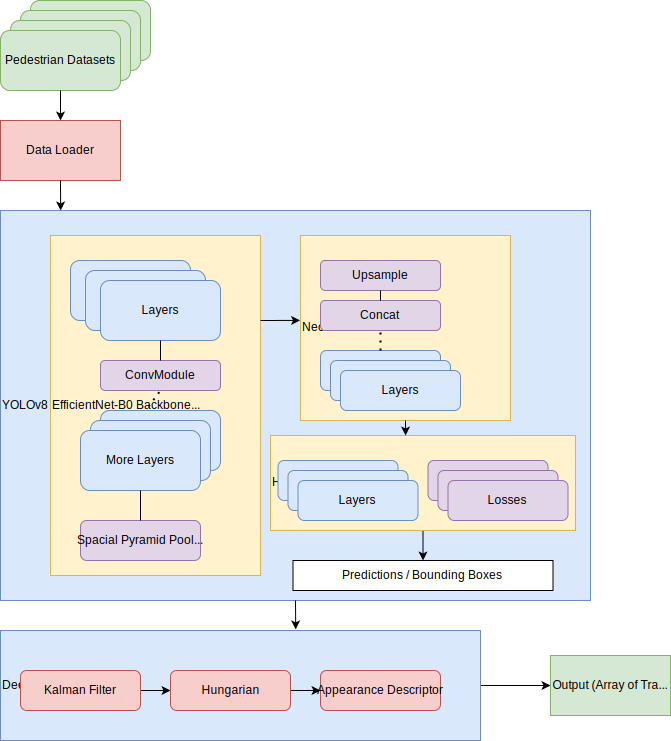
\includegraphics[width=\linewidth]{Figs/arch.png}
    \caption{High-level structure of the pedestrian tracking system.}
    \label{fig:arch}
\end{figure}

\subsection{Tracking}
For tracking, we integrate Deep SORT (Simple Online and Real-time Tracking with a Deep Association Metric) to enhance the robustness and accuracy of the system. Deep SORT extends the original SORT algorithm by incorporating appearance information, which helps maintain object identities across frames \citep{Wojke2018deep}.

The key components of Deep SORT include:
\begin{itemize}
    \item \textbf{Kalman Filter:} This component predicts the future positions of tracked objects based on their previous states, accounting for motion dynamics and handling occlusions \citep{Wojke2018deep}.
    \item \textbf{Hungarian Algorithm:} This algorithm solves the assignment problem of matching detected objects to existing tracks by minimizing the overall cost of associations \citep{Wojke2018deep}.
    \item \textbf{Appearance Descriptor:} A pre-trained CNN extracts appearance features from detected objects, distinguishing between similar-looking objects and maintaining consistent identities over time \citep{Wojke2018deep}. This addresses the problem of distinguishing between different pedestrians so that the model does not incorrectly mix trajectories.
\end{itemize}

The combination of YOLOv8 for detection and Deep SORT for tracking enables the identification of pedestrian heads, the drawing of bounding boxes, and the tracking of their trajectories over time. This architecture ensures efficient and accurate detection and tracking, addressing the requirements of real-time pedestrian tracking applications.

\section{Baseline Model}
To benchmark the performance of our proposed deep learning-based approach, we will compare it against a simple baseline model. The selected baseline is a hand-coded heuristic model utilizing basic image processing techniques for detection and tracking.

\subsection{Detection}
The baseline detection model employs background subtraction to identify moving objects. This method involves calculating the difference between the current frame and a reference frame (typically the previous frame) to detect motion. Any significant changes in pixel values are considered potential detections.

\subsection{Tracking}
The baseline model uses a basic centroid tracking algorithm for tracking. This algorithm computes the centroids of detected bounding boxes and matches them between frames based on spatial proximity. If a detected object is close to a centroid from the previous frame, it is assumed to be the same object.

Although this baseline model is simplistic and does not leverage advanced machine learning techniques, it provides a clear point of comparison to demonstrate the improvements offered by our proposed YOLOv8 and Deep SORT approach. The limitations of the baseline, such as sensitivity to lighting changes and occlusions, will underscore the advantages of employing a deep learning-based solution.

\section{Ethical Considerations}
Pedestrian tracking for biometric authentication raises significant ethical concerns regarding privacy invasion, consent, and potential misuse of sensitive data. Continuous monitoring of individuals' movements could violate their privacy rights, especially without explicit consent. Moreover, there's a risk of unintentional bias or discrimination in the model if the training data lacks diversity. This could cause or exacerbate issues of discrimination, such as racial profiling or continued biased data collection. Ensuring transparency, informed consent and robust security measures is essential to mitigate these risks and address ethical concerns effectively. 

\section{Project Plan}
\subsection{Tracking Tasks}
Our group will use a Google Spreadsheet as a responsibility tracker (instead of the table mentioned in the handout). Each task is assigned to at least one \textit{Responsible} and one \textit{Verifier} party. Once the \textit{responsible} party finishes their task, they will notify the assigned \textit{verifier}; the task is completed once the \textit{verifier} reviews the work. in addition, each task will have a \textit{tag} (e.g. software, documentation, research, etc.). Tags facilitate task delegation. Finally, deadlines are either \textit{hard} or \textit{soft}, representing course and internal deadlines.
\begin{figure}[h]
    \centering
    \includegraphics[width=0.75\linewidth]{Figs/task_tracker.png}
    \caption{Task tracker in Google Sheets.}
    \label{fig:task}
\end{figure}
\subsection{Workflow}
We will use GitHub for our code, Google Drive for draft documents/meeting minutes and Overleaf for final documents. GitHub will ensure that prior versions are not lost while allowing parallel work; \textit{verifiers} will review pull requests. Communication will happen over the team Discord server. Weekly meetings are thus virtual and are scheduled on Sunday at 10 PM. 

\subsection{Responsibilities} \label{responsibilities}
\begin{itemize}
    \item \textbf{Project Manager:} Responsible leader who tracks progress, reminds the team of deadlines, takes meeting minutes, thoroughly reads assignment handouts, and provides the final go-ahead on major project submissions.
    \item \textbf{Data Processor: } Leverages experience in data processing to curate and preprocess the training data and may also collect additional data for testing/validation. 

\item \textbf{ML Engineer:} Leverages experience to select initial hyperparameters, defines the structure of the network and trains the model.
\item \textbf{Writer: } Provides \LaTeX typesetting knowledge for formatting documents/presentations, provides final edits, and ensures deliverables adhere to the assignment rubric.


\end{itemize}


\textit{Note that these roles are subject to change; they are meant to give our team a rough idea of our responsibilities.}

\section{Risk Register}

\subsection{Team Member Attrition}

As outlined above in section \ref{responsibilities} we have established roles and tasks for each member. Our team is not likely to lose a member dropping the course. However, we cannot account for unforeseen circumstances. If a situation were to arise where a member was no longer able to carry out their duties, the task tracker would provide an efficient mechanism to reassign duties. Weekly meetings and detailed meeting minutes will ensure that all members are up to date and minimize friction when being assigned another member’s task.

\subsection{Overfitting}

Although the UCY dataset contains multiple scenarios in various locations, over-fitting may still be a concern. Techniques like dropout, weight decay, and early stopping can be employed while training the model. The same UCY dataset can be augmented by applying transforms to the video (e.g. mirroring) or applying filters/noise to simulate different cameras or lighting conditions. Extensive validation with other datasets and benchmarks should be used to check that the model can generalize to other situations; the model can also be trained with further datasets if necessary.

\subsection{Processing Time}

On the free tier of Google Colab runtimes are limited to 12 hours, this paired with Colab's 12GB RAM limit and limited processing capability may pose a challenge when training and testing the model. If this does pose a problem, we will be able to utilize a team member's Nvidia RTX 3090ti with 24 GB of VRAM to train and test the model locally. While training locally requires proper management of local dependencies, it provides an ``unlimited'' runtime. In addition, the superior compute and large memory allow us to process larger batch sizes, ultimately saving time.


\section{Project Repository}

\url{https://github.com/Tonytheiv/APS360}

\label{last_page}

\bibliography{APS360_ref}
\bibliographystyle{iclr2022_conference}

\end{document}
